\documentclass[a4paper,12pt]{article}
\usepackage[left=2.54cm,top=2.54cm,right=2.54cm, bottom=2.54cm,includehead,nofoot]{geometry}
\usepackage{amsmath}
\usepackage[round]{natbib}
\usepackage{amssymb}
\usepackage{setspace} %for double spacing
\usepackage{fancyhdr}
\usepackage{graphicx}
\usepackage{mathtools}
\usepackage{color}

\begin{document}


\begin{titlepage}
    \begin{center}
        \vspace*{1cm}
        
        \textbf{Kinematics of interstellar filaments and its role in star formation}
        
        \vspace{1.5cm}
        
        \textbf{Britta Hansen\footnote{hansen@astro.utoronto.ca}}

        \vspace{0.5cm}

        Supervisor: Prof. Chris Matzner
        
        \vfill
        
        Thesis proposal\\
        November 19, 2014
        
        \vspace{0.8cm}
        
        Department of Astronomy and Astrophysics\\
        University of Toronto\\

        
    \end{center}
\end{titlepage}


\DeclareGraphicsExtensions{.jpg, .png}

%explain sub and supercritical earlier.

\begin{abstract}

Recent observations of the dense interstellar medium - the main locale of star formation - have found that filamentary structure is ubiquitous and that filaments are strongly associated with clusters. As such, there is much speculation on the effects of filaments on star formation and on the initial mass function. For my thesis I will examine the kinematics of filaments, and the role that filaments play in cluster scale star formation. To do this, I will be running numerical experiments with the adaptive mesh refinement code RAMSES, and by tweaking dimensionless parameters I will look for causal relations between the parameters and the simulation outcomes. The parameters will come from analytical work of others, such as Matzner \& Jumper 2014. I will work under the supposition that matter accretes onto clusters via filaments, hoping to answer questions such as ``Can filaments be the primary source of cluster mass accretion?" and ``How do different filamentary properties affect the properties of the cluster, and of the stars formed within?". All of my numerical experiments and simulations will be compared to observations and theoretical expectations.

\end{abstract}

\section{Scientific motivation}

Filamentary structure has been known to exist in parts of the interstellar medium, such as in the Taurus Molecular Cloud I (TMCI), which is one of the nearest star-formation sites \citep{nut08}. Submillimeter and infrared observations made using Spitzer Space Telescope and the SCUBA project at the James Clerk Maxwell Telescope have captured this filamentary structure in molecular clouds. However, the Herschel Space Observatory (namely the Gould Belt survey) has found that this structure is ubiquitous throughout the cold interstellar medium \citep{and10}, which is the primary locale of star formation. Filaments are often found surrounding clusters, and their pervasiveness has led to the observation that prestellar cores form within filaments \citep{arz11}.\\

Due to the strong presence of filaments in star forming regions, it is natural to wonder how filaments affect star formation, if at all. Could filaments quench or expediate star formation, and how? Ultimately, an understanding of filaments could lead to an understanding of the initial mass function (IMF), the lack of which has long plagued the study of star formation. At the smaller scale, single stars are seen to form in discs. This change in morpholpogy with scale, from discs to filaments, implies that there is a change in the fundamental physics behind star formation from individual stars to clusters of stars. This difference could be due to a change in parameters, including the number of Jeans masses or in the Mach number.\\

Throughout this proposal, I will be referring to filaments as being critical, subcritical, or supercritical. This comes from a notion of \cite{im92} (itself based on \cite{ost64}), in which infinite isothermal cylinders have a characteristic mass per unit length in order to be stable. This is the result of integrating the equations of hydrostatic structure out to infinity. Assuming the density profile is as specified by Ostriker, with $r$ being this cylindrical radius:
\begin{align*}
\rho(r) &= \rho_{max} \left(1 + \left(\frac{r}{H_o}\right)^2\right)^{-2}
\end{align*} Where $H_o$ is the scale height given by $\sqrt{\frac{2c_s^2}{\rho_{max} \pi G}}$\\
They then integrate this as such:
\begin{align*}
\ell&= \int_0^\infty 2\pi r \rho(r) dr\\
	&= \frac{2c_s^2}{G}
\end{align*} $\ell$ is the critical mass per unit length. Any greater mass (supercritical) leads to homologous collapse on a free fall timescale. Any less mass (subcritical) and the filament would expand until it reaches equiblirium with the external pressure. This means that ideal isothermal cylinders can be critical regardless of their radius. However, different density profiles will not integrate to this value, nor will this property hold for non-isothermal filaments, filaments supported by magnetic fields or with turbulence.\\

It has been suggested \citep{pal13} %\citep{andre?} %how many years for t_ff for supercriticals?
that the measured column densities imply some of these filaments are supercritical. If supercritical filaments were to collapse on a free fall timescale of approximately 1 Myr or less, and cluster scale star formation is believed to occur on the order of 5 Myr, then how could filamentary structure be pervasive and causal? \cite{tvg12} have done simple analytical calculations to take into consideration the finite length of a filament. They concluded that the global free fall timescale of a uniform cylinder would be increased from the 3D spherical case by its aspect ratio $A=\frac{L}{R}$, where $L$ is the length of the filament and $R$ is its radius. However its local free fall timescale would be unchanged.\\ %For filaments of 0.05pc width and 3pc length, as found in \cite{and10}, this could add an order of magnitude to their collapse time scale, meaning they would actually collapse slower than 3D spherical regions. It is also possible that stellar feedback and weak magnetic fields further prevent the collapse of the filaments.\\

%Cite Gammie Stone Ostriker. 

%inflow creates bounding pressure too, not just turbulence

%Kristoff Federrath, formation (clustered SF with and without outflows. Molecular cloud put into sim in SPH no magnetic fields turbulence had created sheet like structures in cloud, gravity made fil like structures. Saw clue of formation of filaments, which must have been subcritical because they were falling down onto cluster before breaking up locally.

An understanding of filament instability is necessary for an understanding of the formation of dense cores. If infinite isothermal cylinders can be simulated in pressure equilibrium to maintain their criticality, then adding flow of matter along them would change their criticality condition, and could thus make them fragment. In order to produce dense cores and thus form stars, fragmentation is necessary. We must thus understand the circumstances by which a filament would fragment, and deduce how often this happens for realistic filaments. If simulations of filament fragmentation can produce sufficiently numerous dense cores, then we could causally connect filamentary properties to a star formation rate.\\

%is the arxoumanian citation below the correct arz paper?

Measurements of some properties of filaments have been made, such as the characteristic dimensions, density profiles, and velocity dispersions. \citep{fm12}, \citep{arz11}, \citep{pal13} and \citep{hen13} all found characteristic radii of about 0.1pc. Their lengths are typically 3pc \citep{and10} and their density profiles follow Plummer profiles (\citep{nut08} \citep{jml12} \citep{sgk14}). See Figure 1 for an example of a Plummer profile. \\

%\citep{fm12} Expect the timescale of dispersal for a filament of radius $R$ to be the crossing time given by $\frac{\sqrt{3}}{\sqrt{4\pi G \rho}}$.\\

Recently, \cite{arz13} took measurements of the velocity dispersions of filaments in the Cocoon Nebula, Aquila and Polaris interstellar clouds. They divided the filaments (46 in total) into two categories: thermally subcritical filaments were supersonic but with velocity dispersions less than twice the sound speed, and thermally supercritical, in which the velocity dispersion scaled roughly as the square root of the column density $\sigma_{tot} \propto \Sigma^{0.5}$. The latter are believed to be self-gravitating, while the thermally subcritical filaments were thought to be unbound.\\

The properties of filaments which are expected to play a role in determining fragmentation rates include their density profiles, the presence of magnetic fields and the presence of turbulent motions. The Plummer density profile is given by
\begin{align}
n(r) = n_{flat}\left(\frac{R_{flat}}{\sqrt{R_{flat}^2 + r^2}}\right)^\eta
\end{align} where $n_{flat}(r)$ is the density at the axis of symmetry, $R_{flat}$ is the scale of the region in which the density is nearly uniform, and $\eta$ is a power law slope, and $r$ is still the cylindrical radius. In Plummer's original work \citep{plu1911}, the power law slope was 5, but some authors \citep{nut08} treat $\eta$ as a free parameter. This profile seems to match observations and gives an excellent fit. Though many agree on the functional form of the density profile, it has yet to be determined what the power law slope and flat constant values are, and by how much they can vary. \\

\cite{fri13} found minimum mass accretion rates of $2-5M_\odot Myr^{-1}$ along a filament in Serpens South. \cite{kir13} estimate accretion rate of $28 M_\odot Myr^{-1}$ onto a central cluster along a filament also in Serpens South. If mass is accreting onto filaments, but not homogenously, this could disrupt the density profile of the filament, and thus produce gravitational instabilities within a filament. A flow of mass would also, on the other hand, increase the turbulence, and thus add more support via turbulent pressure.\\

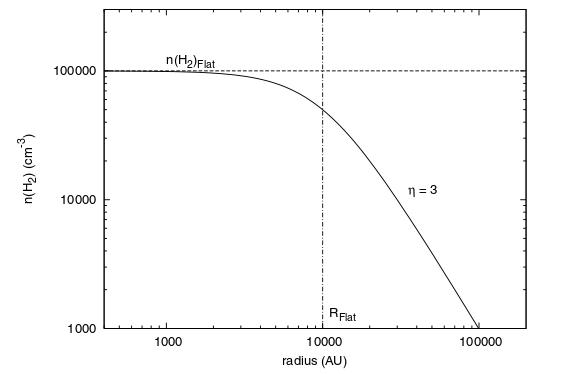
\includegraphics[scale=0.75,natwidth=660,natheight=471]{plummer} \\ {\centering{\singlespacing \tiny 	Fig. 1: Plummer-like profile used in \cite{nut08}. Here they had $\eta =3$, $n(H_2)_{flat} = 10^5$cm$^{-3}$ and $R_{flat} = 10^4$au.}}\\

Some have suggested magnetic fields are necessary to slow the collapse of filaments \citep{pal13}. Larson has analytically shown that for toy models, magnetic fields indeed can inhibit collapse of a filament \citep{lar85}. \cite{pal13} pointed out that there are smaller filamentary structures - striations - in the TMC, orthogonal to the primary filament B211. With dust polarization maps, they concluded that the striations are somewhat aligned with the magnetic field of $25 \mu$G, and thus suggested that magnetic fields could determine the morphology of the clouds. They also speculated that the primary filament could be accreting mass along the field lines via these striations. The Intermediate Planck results recently looked at polarization data for 3 filaments each about 3pc in length \citep{planck33}. They found that the filament L1506 in the TMC had its background magnetic field parallel to the filament. Although there is very little polarization data available for interstellar filaments, this single counterexample leads one to believe that mass accreting via striations aligned with the magnetic field might not be a necessary condition for the maintenance of interstellar filaments. Similar striations have also been seen in the Pipe Nebula \citep{per12}. Figure 3 depicts such a filament. \\

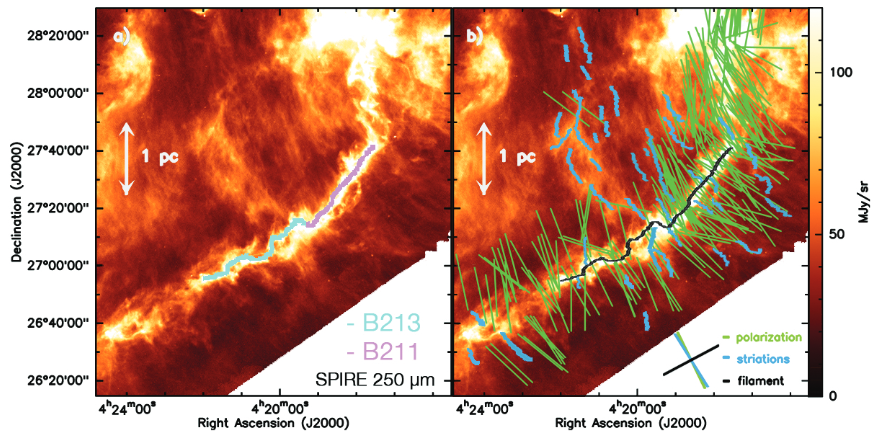
\includegraphics[scale=0.5,natwidth=898,natheight=567]{Herschel_Taurus_B211}\\ {\centering{\singlespacing \tiny 	Fig. 2: The filaments B211 and B213 in the TMC, as seen by Herschel. Image taken from \citep{pal13}}}\\ \\

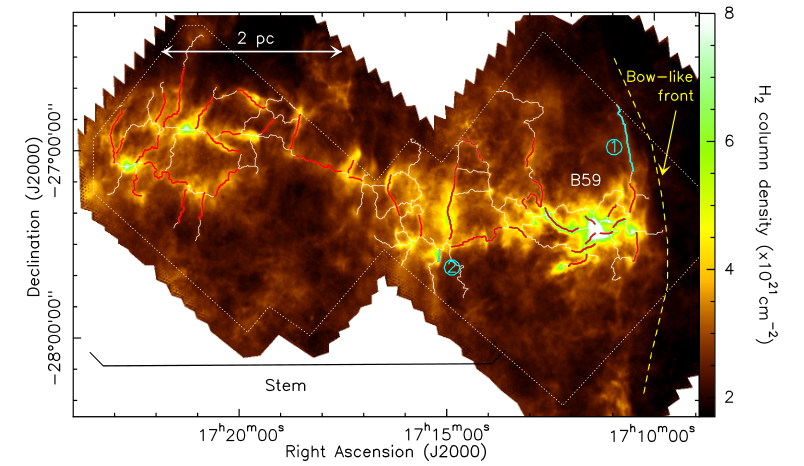
\includegraphics[scale=0.5,natwidth=867,natheight=583]{Pipe_Nebula} \\ {\centering{\singlespacing \tiny 	Fig. 3: Column density map from Herschel data of the Pipe Nebula. Red lines are filaments traced using an algorithm called DisPerSE. Image taken from \citep{per12}}}

\section{Course of action}

For my thesis I propose to investigate the role of filaments in cluster-scale star formation with numerical surveys. The work will use dimensionless parameters motivated by the analytical work of others such as \citep{mat14} and \citep{im97}, in which simulations will be run with the parameters held fixed, so that each run allows for time evolution with the parameters as initial conditions. \\

%REWORK> DESCRIBE PARAMS IN WORDS. WHY DO THEY HAVE PHYSICAL MEANING? DO I HAVE EXPECTATIONS OF HOW THEY"LL EVOLVE?, the virial parameter (3), and the ratio of mass accretion to velocity dispersion (4). This last parameter comes from \citep{mat14}. The specific forms of these parameters is given as follows:

Some useful quantities required below include:\\

The Jeans mass
\begin{align*}
M_J &= \frac{\pi c_s^3}{6\sqrt{G^3\rho_{max}}}
\end{align*} where $\rho$ is the central density within the filament.\\

The local free-fall timescale for the filament
\begin{align*}
t_{ff} &= \sqrt{\frac{3\pi }{32G\rho_{max}}}
\end{align*}\\

The critical mass per unit length for filaments
\begin{align*}
\ell=\frac{2c_s^2}{G}
\end{align*}

\subsection{Studies of a single infinite filament}

The first simulations will be performed on single, static, infinite isothermal filaments as a proof of concept and a code test. I will attempt to make such filaments `stand still' in that they are critical: neither expanding nor collapsing.  I then will add turbulence to the filament and eventually a magnetic field oriented paerpendicular to the filament, and I will see how they affect the criticality. For filaments rendered supercritical, I will measure the timescale of their collapse. As mentioned in the motivational section, it is expected that turbulence, magnetic fields, and mass flow would all increase the criticality condition of the filaments, thereby making them subcritical. They would thus expand until they reach pressure equilibrium with the surrounding medium.\\

Throughout these simulations, I will be monitoring several dimensionless parameters including the actual mass per unit length of the filament divided by the critical mass per unit length
\begin{align}
\eta &=\frac{\rho_{max}\pi R_f^2}{\ell}
\end{align} This quantity is useful when magnetic fields and turbulence are added to the picture, since it will tell us how they affect the criticality of the filament.\\

%The ratio of two possible crossing times for the filament
%\begin{align}
%n_2&=\frac{\sqrt{3}c_s}{\sqrt{4\pi G\rho}R_f}
%\end{align} This is the crossing time for a uniform sphere, divided by the sound crossing time along the radius of the filament. WHY %WOULD YOU LOOK AT THIS?\\

%The ratio of dynamical viscosities of the filament 
%\begin{align}
%n_3 &= \frac{c_s \rho R_f^2}{\dot{M}}
%\end{align} $c_s\rho R_f$ is the inertial force per cross-sectional area. $\frac{\dot{M}}{R_f}$ is like a dynamical force per unit area. This will help me understand the effects of mass accretion of the criticality of the filament. It is expected that an increased mass flow through the filament would increase the amount of turbulence in the filament, and thus add support. Increased turbulence would also mean the filament would expand if it began as critical, so I would expect this parameter to increase. As well, if a filament had shear, the sound crossing time would be unchanged, but the mass accretion rate would have a discontinuity long the radial direction. \\

Once the effects of mass flow and magnetic fields on a toy filament are understood, I will then focus on the effects of the density profile on filament shape and behaviour. These will still be single infinite isothermal filaments, now with a steady flow of mass. Each simulation will begin with critical filaments but with different parameters from the Plummer profile given in equation (5) above. I wish to answer whether different density profiles could affect the mass accretion rate onto a cluster. This will be accomplished by measuring the mass accretion rate profile through the boundary.\\

I am also interested in giving a filament shear along the axis of symmetry, and examining how the shear changes the shape of the filament with time, as well as its density profile. I can measure the timescale of their collapse or fragmentation, and compare this to the timescales given by Inutsuka and Miyama. Does the flow rate affect the timescale of collapse for a supercritical filament? Can high mass flows cause fragmentation? How high?

\subsection{Multiple filaments connecting at a node}

Once this is set up and I am confident that my singular filaments are realistic, I will add multiple filaments connecting into a node, the node acting as a cluster. My focus will be on the possibility that filaments feed the cluster's mass accretion rate, in that matter flows down the filaments into the cluster.\\

This project intends to bridge the thesis work of former doctoral student Kaitlin Kratter \citep{kra10}, (a numerical parametre study of accretion in single star systems) with the current work of PhD student Peter Jumper (star formation at the cluster level). Some questions I may attempt to answer include ``Why are discs important at the individual star level, but not the level of star clusters?'' and ``What sets the mass scale of the cluster?''.\\

Throughout the simulations, there are several things I will check for to see if the simulation is realistic and matching observations:

\begin{itemize}
\item Do the filaments maintain their 0.1 pc radial scale, as observed by \cite{fm12}, \cite{arz11} and \cite{hen13}? 
\item Does the line density grow quadratically with time, as predicted by \cite{mat14}?
\item Is the mass accretion rate by this mode sufficiently high to give the expected rates of star formation?
\item Do filaments collapse too quickly (less than a few Myr) in order to be pervasive?
\end{itemize}

Some of the parameters that I will investigate and monitor throughout the simulations are as follows.\\

The virial parameter is the ratio of kinetic and gravitational potential energies
\begin{align}
\alpha &= \frac{5\sigma_c^2R_c}{GM_c}
\end{align} The virial parameter is expected to remain on the order of unity in molecular clouds and self-gravitating regions (\citep{bm92} \citep{kau13}). $R_C$, $\sigma_c$ and $M_C$ will all change in time.\\

The turbulent Mach number
\begin{align}
M &= \frac{\sigma_c}{c_s}
\end{align} This determines the degree of incompressibility of a flow. A low Mach number would indicate a lack of turbulence, and thus a nearly-laminar flow.\\

The dimensionless accretion rate
\begin{align}
\xi &= \frac{\dot{M}G}{\sigma_c^3}
\end{align} \cite{mat14} expect $\xi$ to be of order unity, but are not very certain of its value, thus it is fruitful to measure it. Indeed, one might expect that as the accretion increases, more turbulence is injected, thereby justifying the near-order-unity anticipation.\\

%The number of filament Jeans masses per mass accreted in a cluster free-fall time.
%\begin{align}
%n_7 &= \frac{\pi c_s^3}{6 G^{\frac{3}{2}}\rho^{\frac{1}{2}}\dot{M}t_{ff}}\\
%	&= \frac{c_s^3\sqrt{8M_c}}{\dot{M}\pi G\sqrt{\rho R_c^3}}
%\end{align} \\

%The total cluster mass divided by the mass accreted in a free fall time
%\begin{align}
%n_8 &= \frac{\sqrt{8M_c^3 G}}{\dot{M}\pi \sqrt{R_c^3}}
%\end{align}\\

%13. Ratio of dynamical viscosities: inertial force of filament (per area) divided by inertial force of cluster (per area).
%\begin{align}
%n_9 &= \frac{c_s\rho R_fR_c^2}{\sigma M_c}
%\end{align}\\

%14. Ratio of dynamical viscosities: inertial force of cluster (per area) divided by inertial force of filament (per area).
%\begin{align}
%n_10 &= \frac{\sigma M_c R_f}{R_c^2 \dot{M}}
%\end{align}

\subsection{Simulation methodology} 

I determine the input parameters before each run. Once a simulation is complete, I will compute the outputs of the code (see section 2.5) This will allow me to measure the dimensionless parameters given in equations (2) through (12). I can then map the values of these parameters for each simulation. For instance, here is a plot from \cite{kra10}, in which the values of parameters $\xi$ and $\Gamma$ are measured after each simulation.

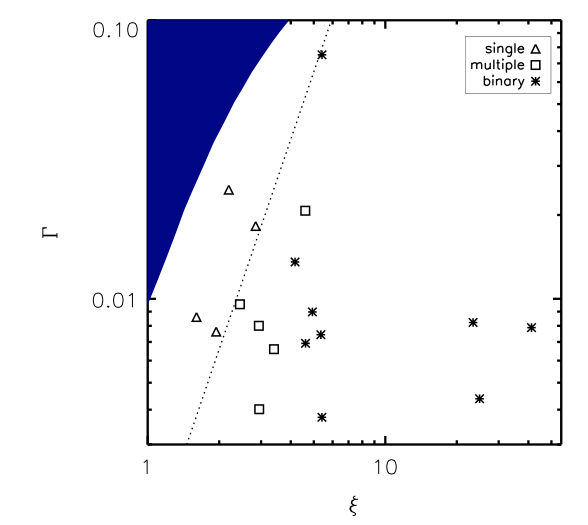
\includegraphics[scale=0.5,natwidth=588,natheight=525]{Kratter} \\ {\centering \singlespacing \tiny 	Fig. 4:  A map of measured ratios of dimensionless parameters $\xi$ and $\Gamma$ taken from \cite{kra10}. These ratios were measured from simulation outputs, and can be used to identify regions (ratios) in which specific physical phenomena occured, such as the formation of a binary star system.}\\

Once a map such as this has been constructed, I can begin to causally connect phenomena of the simulation outcomes to the region on the map. For \citep{kra10}, it was noticed that binary stars formed consistently within a particular region of this map (for a particular ratio of $\xi$ to $\Gamma$), and single stars in others. Some of the phenomena I could look for in my simulations may be the number of fragments of a filament or the number of sink particles formed within the cluster.

\subsection{The code}

RAMSES is an MHD code using adaptive mesh refinement (AMR) \citep{tey02}. It uses a space-filling curve to refine details, as compared to traditional AMR codes which use a cartesian mesh. The advantage of the space-filling curve is an improved load balance between GPUs when parallel computing. The code is publically available and written in Fortran90.\\

There are several reasons I have chosen to use RAMSES as my primary code for these simulations. AMR codes as opposed to SPH (smooth particle hydrodynamics) tend to do a better job with hydrodynamics and shocks. Since these are hydro simulations which could include feedback and turbulence, it is imperative to be able to resolve the effects. I might also like to add magnetic fields later, which RAMSES can do. The public availability of the code make it accessible and RAMSES has particle data in which the particles move separately from mesh, therefore we can have both gas and stars.\\

It is also necessary to use a 3D simulation throughout this work. Although a single cylinder is a one dimensional object, I want to observe mass accretion onto the filament in 3D. I need to be certain I'm not just looking at a cross section of a sheet; it is expected that sheets would have different free fall timescales. Eventually I will have multiple filaments in a three dimensional geometry. \\

Resolution tests will determine if my results have converged. We may wish to do a code comparison, and are considering FLASH as a secondary code for this purpose. FLASH is also a publicly available AMR code, but it uses a Cartesian grid with sink particles. 

\subsection{Extracting data from the simulation results}

The particle output data from RAMSES includes their velocities, masses, birth time, metallicities, and number. The AMR output data includes density, velocity field, pressure, and gravitational acceleration. From this, some quantities are immediate to compute, such as the density and pressure profiles of a region. Other outputs include measures of the kinetic energy and the error on energy conservation.\\

In order to determine the velocity dispersion in RAMSES we can subtract the bulk motion for the velocity fields, and then measure the mass of fluid within a turblent zone. We can then divide the kinetic energy of this region by the mass to get approximately the square of the velocity dispersion.\\

\subsection{Further work: filament formation}

Once we have completed some of the more controlled numerical experiments would be interested in exploring the creation of filaments within a molecular cloud. We don't have a complete plan at this point therefore this topic is only going to be explored time permitting. Time permitting, some of the simulations could have as objective to verify whether striations caused by magnetic fields are consistent with filamentary mass infall rates of 2-5 $M_{\odot}$Myr$^{-1}$\citep{fri13}. They will be performed by putting a magnetic field of strength on the order of 0.5$\mu$G orthogonal to the filament, and outfitting the filament with a Plummer-like profile and a flow of mass. Then I will observe how the magnetic field affects the density profile and the mass infall rate by varying the field strength.  

Since there is some evidence of mass accreting onto filaments along magnetic field lines (\citep{fri13}, \citep{kir13}), for the sake of filament formation and maintenance I am interested in adding small lower density filaments feeding into the primary filament. The expected molecular column density of a striation is about $2$x$10^{21} cm^{-2}$, over an order of magnitude lower than for the main filament \citep{pal13}. I will investigate whether such striations add substantial turbulence to the primary filament, and whether they create density inhomogeneities. Could they be sufficient to maintain a filament which has significant mass loss?\\

\subsection{Progress}

Most work so far has been setting up and understanding how the RAMSES code functions. The code comes with a test suite; I have been trying to get each of the tests to work, and then tweaking their input parameters to understand how these parameters function and affect the outcome. I have thus been learning how to use the Python module Pymses, in order extract the binary output from the program. From there I have been playing with matplotlib and Visit in order to make movies and plots of my simulation data.\\

I am presently trying to write my own initial conditions files rather than using the supplied files. This should allow me to make more complex shapes and flows than what is given in the test suite. I am also checking my single simulated filaments to see if their mass per unit length follows the critical behaviour as expected from \cite{im92}

\section{Schedule} %order, not dates

\textbf{Present:} Continue to run tests with the RAMSES code and attempt to achieve anything resembling realistic initial conditions and isothermal filaments in pressure equilibrium. Check that my supercritical isothermal filaments collapse, and subcritical ones expand. Measure the timescale of collapse for supercritical filaments.\\ \\ \textbf{Spring 2015:} Give the filament a flow, as though feeding into a cluster. Vary the Plummer profile parameters and see how this affects the shape and mass accretion rate. Measure the timescales for collapse. Time permitting, give it shear. Now put a magnetic field orthogonal to the filament and measure the effects thereof and density profiles, collapse timescales, and criticality.\\ \\\textbf{Late 2015:} Simulate flow along multiple filaments into a cluster (read: spherical node). Focus on the variation in line density. With ``supercritical'' filaments feeding into a cluster, under what timescale do they collapse? Could this quench star formation? How do different mass accretion rates affect the properties of the cluster? Continue to explore the parameter space, varying the mass accretion rate onto the cluster.\\ \\ \textbf{Mid 2016:} Add more filaments to the simulation. Even if the mass accretion rate is kept the same as with fewer filaments, are there the same number of sink particles created? How does this affect the velocity dispersion? Add striations feeding into a single filament. How do they affect the internal properties of the filament?\\ \\ \textbf{Spring 2017:} Begin working on thesis text. Try to incorporate a global magnetic field into the cluster-scale simulation \\ \\ \textbf{Fall 2017:} Submit finished thesis to committee. Defend at the end of autumn 2017.

%MODELS
%MARTIN & FISCHERA isothermal self-gravitating infinite cylinder in pressure equilibrium with the ambient medium. Their gravitational state is characterized by the ratio fcyl of their mass line density to the maximum possible value for a cylinder in a vacuum.

%HEITSCH: 

%HENNEBELLE: 

\singlespacing
\bibliographystyle{plainnat}
\bibliography{bibliography}

\end{document}
